\documentclass{article}
\usepackage{algorithm}
\usepackage{algpseudocode}
\usepackage{amsmath}
\usepackage{amsfonts}
\usepackage{graphicx}
\usepackage{listings}
\title{Simple Grid World Environment Tutorial}
\author{Your Name}
\date{\today}

\begin{document}
\maketitle

\section{Introduction}
In this tutorial, we will discuss a simple grid world environment that can be used for reinforcement learning. The environment consists of a grid with three states: S1, S2, and a goal state G. The agent can take two actions: Left and Right. The goal of the agent is to reach the goal state G from the starting state S1 while maximizing its total reward.

\section{Environment Initialization}
\begin{algorithm}
\caption{Initialization of the Simple Grid World Environment}\label{alg:init}
\begin{algorithmic}[1]
\State $\text{observation\_space} \gets \text{Discrete}(3)$ \Comment{3 states: S1, S2, G}
\State $\text{action\_space} \gets \text{Discrete}(2)$ \Comment{2 actions: Left, Right}
\State $\text{state} \gets 0$ \Comment{Starting state S1}
\State $\text{done} \gets \text{False}$

\State Define transition dynamics $\text{P}$ and the grid world $\text{grid}$ \Comment{See code for details}
\end{algorithmic}
\end{algorithm}

\section{Resetting the Environment}
\begin{algorithm}
\caption{Resetting the Environment}\label{alg:reset}
\begin{algorithmic}[1]
\State $\text{state} \gets 0$ \Comment{Reset to starting state S1}
\State $\text{done} \gets \text{False}$
\State \Return $\text{state}$
\end{algorithmic}
\end{algorithm}

\section{Taking a Step in the Environment}
\begin{algorithm}
\caption{Taking a Step in the Environment}\label{alg:step}
\begin{algorithmic}[1]
\State $\text{transitions} \gets \text{P[state][action]}$
\State $\text{prob}, \text{next\_state}, \text{reward}, \text{done} \gets \text{transitions[0]}$ \Comment{Assuming deterministic transitions}
\State $\text{state} \gets \text{next\_state}$
\State $\text{done} \gets \text{done}$
\If{$\text{done}$ \textbf{and} $\text{reward} \neq 10$}
    \State $\text{reward} \gets -10$ \Comment{Penalize for reaching a non-goal terminal state}
\EndIf
\State \Return $\text{state}, \text{reward}, \text{done}, \{\}$
\end{algorithmic}
\end{algorithm}

\section{Rendering the Environment}
The render method is used to visualize the current state of the environment. The grid world is represented as a 2D array where each cell represents a state. The agent's position is indicated by a value of 1 in the grid.

\begin{figure}[htbp]
\centering
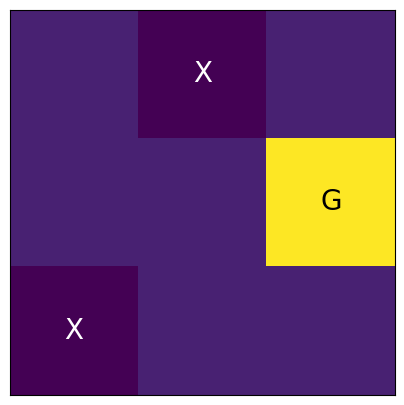
\includegraphics[width=0.5\textwidth]{gridworld.png}
\caption{Visualization of the Grid World Environment}\label{fig:gridworld}
\end{figure}
\section{Implementation}
1. create a new notebook 
2. import the required library 
\begin{lstlisting}
import matplotlib.pyplot as plt
import numpy as np
import gym

\end{lstlisting}
add a new class 
\begin{lstlisting}
class SimpleGridWorldEnv(gym.Env):
    def __init__(self):
        self.observation_space = gym.spaces.Discrete(3)  # 3 states: S1, S2, G
        self.action_space = gym.spaces.Discrete(2)       # 2 actions: Left, Right
        self.state = 0  # Starting state S1
        self.done = False

        # Define transition dynamics
        self.P = {
            0: {0: [(1.0, 0, -1, False)], 1: [(1.0, 1, -1, False)]},  # Transition from S1
            1: {0: [(1.0, 0, -1, False)], 1: [(1.0, 2, 10, True)]},   # Transition from S2
            2: {0: [], 1: []}  # Terminal state G
        }

        # Define the grid world
        self.grid = np.array([[0, -1, 0], [0, 0, 10], [-1, 0, 0]])

    def reset(self):
        self.state = 0  # Reset to starting state S1
        self.done = False
        return self.state

    def step(self, action):
        transitions = self.P[self.state][action]
        prob, next_state, reward, done = transitions[0]  # Assuming deterministic transitions
        self.state = next_state
        self.done = done
        if done and reward != 10:  # If the agent did not reach the goal state
            reward = -10  # Penalize for reaching a non-goal terminal state
        return self.state, reward, self.done, {}

    def render(self):
        grid_with_agent = np.copy(self.grid)
        grid_with_agent[self.state // 3, self.state % 3] = 1  # Place agent in the grid
        return grid_with_agent
\end{lstlisting}
\end{document}
